
\refstepcounter{Exercise}
\clearpage\subsection*{\theExercise CGIを使ってOpenJtalkに読み上げをさせよう}
\addtocounter{Exercise}{-1}\refstepcounter{Exercise}\label{E:Jtalk}
% \clearpage\subsection*{CGIを使ってOpenJtalkに読み上げをさせよう}

考え方

ウェブページから読み上げさせたい文章を受け取って、OpenJtalkにCGIから読み上げをさせよう。

まずは、試してみよう。

ブラウザを開いて

localhost:3000/jtalk.html

にアクセスをしてみよう。

%
%ぶらうざで開いた画面n
%koyaman
%September 20, 2019 2:50 AM


\centering
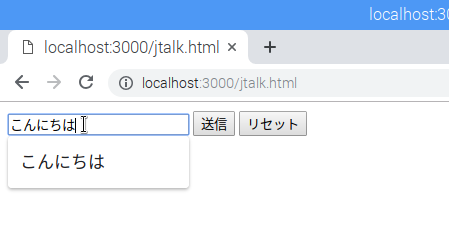
\includegraphics[width=0.85\textwidth]{text07-img/ome7-img056.png}
\flushleft

テキストボックスに読み上げさせたい文章を入れて送信をしてみよう。送信を押すとCGIプログラムへ文章が送られ、OpenJtalkで音声合成をします。


\bigskip

結果をウェブページのaudioタグ(音声を再生するタグ)へ渡して\ruby{再生}{さいせい}をします。

%
%
%音声ファイルを再生する画面のスクショ
%koyaman
%September 20, 2019 2:50 AM


\centering
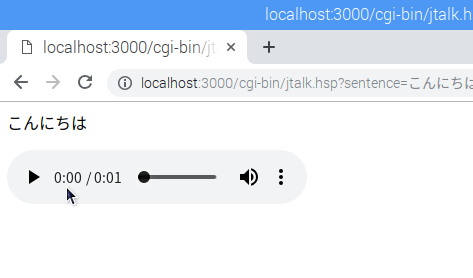
\includegraphics[width=0.85\textwidth]{text07-img/ome7-img057.png}
\flushleft

\clearpage
プログラム解説

{\textasciitilde}/07/www/jtalk.html





\begin{table}[htbp]
    \centering
    % \caption{文字タイプ表}
    \begin{tabular}{|l|}
        \hline
        
        1. {\textless}!DOCTYPE html{\textgreater}\\ 
        2. {\textless}html{\textgreater}\\
        3. {\textless}head{\textgreater}\\
        4. \ \ \ \ {\textless}meta charset={\textquotedbl}utf-8{\textquotedbl}{\textgreater}\\
        5. {\textless}/head{\textgreater}\\
        6. {\textless}body{\textgreater}\\
        7. \ \ \ \ {\textless}form action={\textquotedbl}cgi-bin/jtalk.hsp{\textquotedbl} method={\textquotedbl}GET{\textquotedbl}{\textgreater}\\
        8. \ \ \ \ \ \ \ \ {\textless}input type={\textquotedbl}text{\textquotedbl} name={\textquotedbl}sentence{\textquotedbl}{\textgreater}\\
        9. \ \ \ \ \ \ \ \ {\textless}input type={\textquotedbl}submit{\textquotedbl} value={\textquotedbl}送信{\textquotedbl}{\textgreater}\\
        10. \ \ \ \ \ \ \ \ {\textless}input type={\textquotedbl}reset{\textquotedbl} value={\textquotedbl}リセット{\textquotedbl}{\textgreater}\\
        11. \ \ \ \ {\textless}/form{\textgreater}\\
        12. {\textless}/body{\textgreater}\\
        13. {\textless}/html{\textgreater}\\
        
        \hline
    \end{tabular}
\end{table}




\bigskip


\bigskip



\bigskip

7〜11行目では、CGIようにフォーム(form)を用意しています。

文字を入れるテキストボックスが一つと送信用のボタンが一つ、テキストボックスをリセットするボタンが一つあります。

%
%スクリーンショット
%ブラウザでjtalk.htmlを開いた画像
%koyaman
%September 19, 2019 11:59 PM


7行目の

{\textless}form action={\textquotedbl}cgi-bin/jtalk.hsp{\textquotedbl}
method={\textquotedbl}GET{\textquotedbl}{\textgreater}

action=”cgi-bin/jtalk.hsp”

はフォームに入力された情報をを受ける(処理する)CGIプログラムを指定します。

method=”GET”

はクエリストリングとしてフォームの情報をCGIに渡すことを指示しています。

8行目の

{\textless}input type={\textquotedbl}text{\textquotedbl} name={\textquotedbl}sentence{\textquotedbl}{\textgreater}

では、テキストボックスを作っています。

name=”sentence”

はクエリストリングの名前を指定します。入力された文字列が値となります。ちなみにsentenceとは日本語にすると”文章”という意味になります。

例えば、テキストボックスに

“こんにちは”とテキストボックスに入力され、送信された場合

\clearpage
\bigskip



\centering
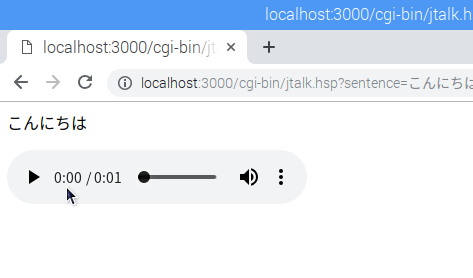
\includegraphics[width=0.85\textwidth]{text07-img/ome7-img057.png}

\centering
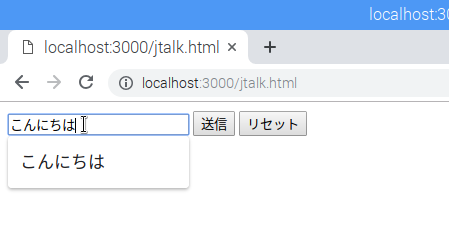
\includegraphics[width=0.85\textwidth]{text07-img/ome7-img056.png}
\flushleft


\bigskip

%
%スクショ
%こんにちはとテキストボックスに
%koyaman
%September 20, 2019 12:04 AM


ウェブサーバにこのような要求を出します。

IPアドレス:3000/cgi-bin/jtalk.hsp?sentence=こんにちは

実際には”こんにちは”という文字列はURL内ではある\ruby{規則}{きそく}に\ruby{沿}{そ}って記号、数値に変換されています。

このことをパーセントエンコーディングといいます。CGIプログラムにクエリストリングが渡される前にウェブサーバは記号、数値に変換された文字列をもとに戻します。よって、プログラム内では入力された文字列と同じものを扱うことができます。

{\textasciitilde}/07/www/cgi-bin/jtalk.hsp


\begin{table}[htbp]
    \centering
    % \caption{文字タイプ表}
    \begin{tabular}{|l|}
        \hline
        
        1. \#include {\textquotedbl}hsp3cl.as{\textquotedbl}\\ 
        2. \#include {\textquotedbl}jtalk.as{\textquotedbl}\\
        3. \#include {\textquotedbl}cgi.as{\textquotedbl}\\
        4. \\
        5. mes {\textquotedbl}Content-type: text/html{\textbackslash}n{\textquotedbl}\\
        6. mes {\textquotedbl}{\textless}html{\textgreater}{\textless}head{\textgreater}{\textless}meta charset={\textbackslash}{\textquotedbl}utf-8{\textbackslash}{\textquotedbl}{\textgreater}{\textless}/head{\textgreater}{\textless}body{\textgreater}{\textquotedbl}\\
        7. \\
        8. getqueryval {\textquotedbl}sentence{\textquotedbl}, sentence\\
        9. jtsave sentence, wav\_file\\
        10. mes {\textquotedbl}{\textless}p{\textgreater}{\textquotedbl} + sentence + {\textquotedbl}{\textless}/p{\textgreater}{\textquotedbl}\\
        11. \\
        12. mes {\textquotedbl}{\textless}audio src={\textbackslash}{\textquotedbl}{\textquotedbl} \ + wav\_file + {\textquotedbl}{\textbackslash}{\textquotedbl} type={\textbackslash}{\textquotedbl}audio/wav{\textbackslash}{\textquotedbl} controls{\textgreater}{\textquotedbl}\\
        13. mes {\textquotedbl}{\textless}/body{\textgreater}{\textless}/html{\textgreater}{\textquotedbl}\\
        14. end\\
        
        \hline
    \end{tabular}
\end{table}






\bigskip

8行目でjtalk.htmlのフォームの

{\textless}input type={\textquotedbl}text{\textquotedbl} name={\textquotedbl}sentence{\textquotedbl}{\textgreater}

に入っている値を取り出しています。取り出した値はsentence変数へ入れています。

9行目の

jtsave sentence, wav\_file

はsentence変数の中の文字列を音声合成して音声ファイルのファイル名をwav\_file変数へ入れています。

12行目の

mes {\textquotedbl}{\textless}audio src={\textbackslash}{\textquotedbl}{\textquotedbl} \ + wav\_file +
{\textquotedbl}{\textbackslash}{\textquotedbl}
type={\textbackslash}{\textquotedbl}audio/wav{\textbackslash}{\textquotedbl} controls{\textgreater}{\textquotedbl}

	{\textless}audio{\textgreater}タグは音声ファイルを再生することができます。

src=”ファイル名”

では、再生するファイルを指定します。指定するファイルはドキュメントルート以下にないといけません。つまり、ドキュメントルートである{\textasciitilde}/07/wwwの中にある必要があります。

jtsave命令で作った音声ファイルは{\textasciitilde}/07/www/tmpの中にあります。ファイル名はwav\_file変数に入っています。

“
“の中で”を使うには{\textbackslash}”のように書きます。

type=”audio/wav”

では、音声ファイルの種類を決めます。jtsave命令が作る音声ファイルの場合は、

type=”audio/wav”にします。

controlsをつけると、再生ボタン、ミュートボタンなどが表示されます。

再生ボタンを押すと音声合成した音声ファイルが再生されます。

\clearpage
\refstepcounter{Question}\theQuestion\label{Q:Jtalk}

{\bfseries
	”おはようございます””こんばんは””ありがとうございます”を読ませてみよう。}


\bigskip

できる人は自分の自己紹介ページに({\textasciitilde}/07/www/index.html)に作ったフォームを変更して、こちらからCGIプログラムを起動するようにしましょう。

\ HINT: jtalk.htmlを参考にしてください。